%\addcontentsline{toc}{chapter}{Falcon 9 v1.1 flight performance}\label{ch:Falcon9}
\chapter{Falcon 9 v1.1 flight performance}
\label{ch:Falcon9}

In order to develop relevant solutions to  problems in industry, it is important to have an understanding of what the real world challenges faced by the receiver are. A thorough understanding of the real world challenges allows accurate simulations analysis to be carried out.

\begin{figure}[!htb] 
    \centering
    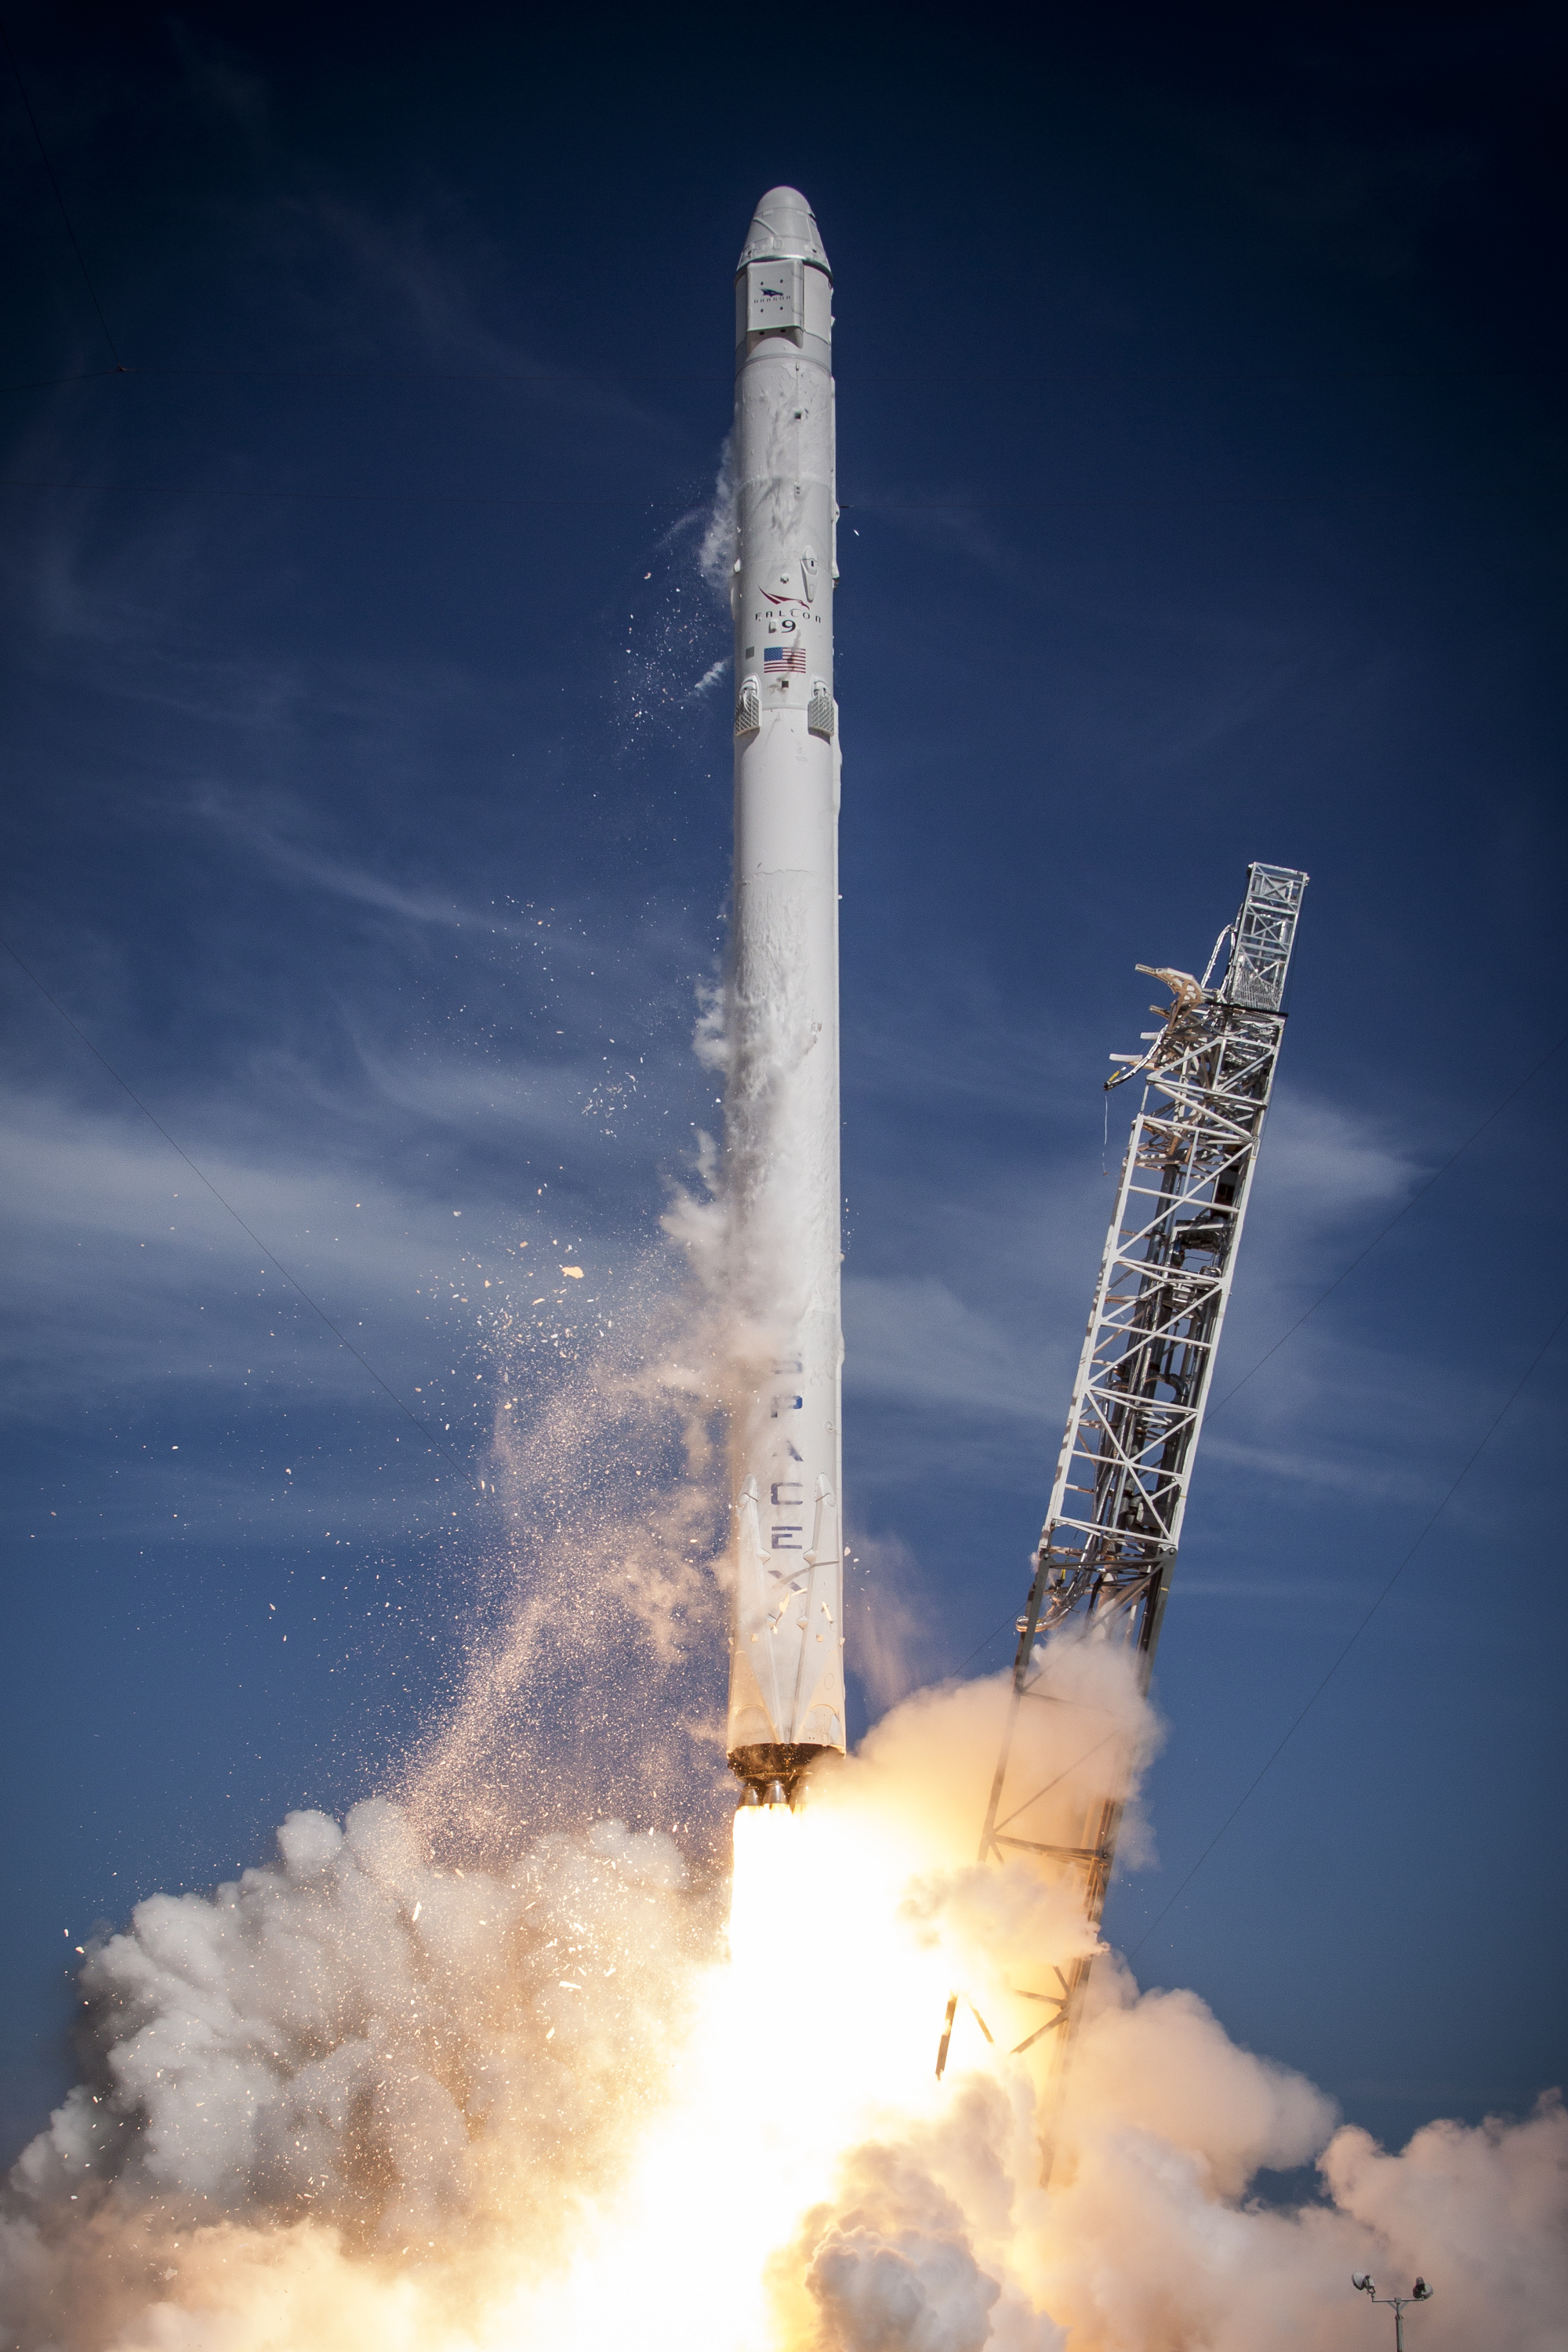
\includegraphics[width=0.8\textwidth]{Falcon9/crs6_launch_center.jpg} 
    \caption{CRS-6 Launch. At launch, the rocket has an initial acceleration of $\approx$ 1.2g. Image from \cite{SpaceXPhotos}.}
    \label{fig:Falcon9}
\end{figure}


\begin{table}[!htb]
\centering
\begin{tabular}{|l|l|}
\hline
\rowcolor[HTML]{C0C0C0} 
Parameter                   & Value     \\ \hline
Stage thrust (Sea level)    & 6,806kN   \\ \hline
\rowcolor[HTML]{EFEFEF} 
Stage thrust (Vacuum)       & 7,426kN   \\ \hline
Number of engines           & 9         \\ \hline
\rowcolor[HTML]{EFEFEF} 
Fuel flow rate (per engine) & 250kg/s   \\ \hline
Burn time (9 engines)       & 155.5 s   \\ \hline
\rowcolor[HTML]{EFEFEF} 
Burn time (7 engines)       & 18.7 s    \\ \hline
Fuel mass                   & 382,750kg \\ \hline
\end{tabular}
\caption{1st stage key statistics.}
\label{tab:1stStageStats}
\end{table}

\begin{table}[!htb]
\centering
\begin{tabular}{|l|l|}
\hline
\rowcolor[HTML]{C0C0C0} 
Parameter                   & Value    \\ \hline
\rowcolor[HTML]{EFEFEF} 
Stage thrust (Vacuum)       & 800kN    \\ \hline
Number of engines           & 1        \\ \hline
\rowcolor[HTML]{EFEFEF} 
Fuel flow rate (per engine) & 250kg/s  \\ \hline
Burn time                   & 296.7 s  \\ \hline
\rowcolor[HTML]{EFEFEF} 
Fuel mass                   & 74,175kg \\ \hline
\end{tabular}
\caption{2nd stage key statistics.}
\label{tab:2ndStageStats}
\end{table}


In order to meet this goal, the Falcon 9 v1.1 rocket was chosen for analysis. This was for a number of salient reasons, At 70M tall, weighing 540 tons at launch and costing \$85M AUD \cite{SpaceXFalcon9}, the Falcon9 v1.1 has performance characteristics that are typical of a modern \ac{LV}. Space Exploration Technology Corporation (SpaceX) who develop, construct and launch the Falcon 9 are more open regarding the technical details of their \ac{LV} than their contemporaries, allowing numerical models of performance to be developed. Finally, the Falcon 9 v1.1 experiences a wide variety of dynamics, including the first stage conducting a "hover slam" or "suicide burn" manoeuvre, the success of which is reliant on accurate position and velocity estimates.

Because the actual flight performance of the Falcon 9 v1.1 is proprietary and confidential, an effort must be made to develop an model which uses publicly disclosed information. In this manner, a model of the performance can be developed, and compared against real world performance of the \ac{LV}.

%\section{Physics model}

\begin{figure}[!htb] 
    \centering
    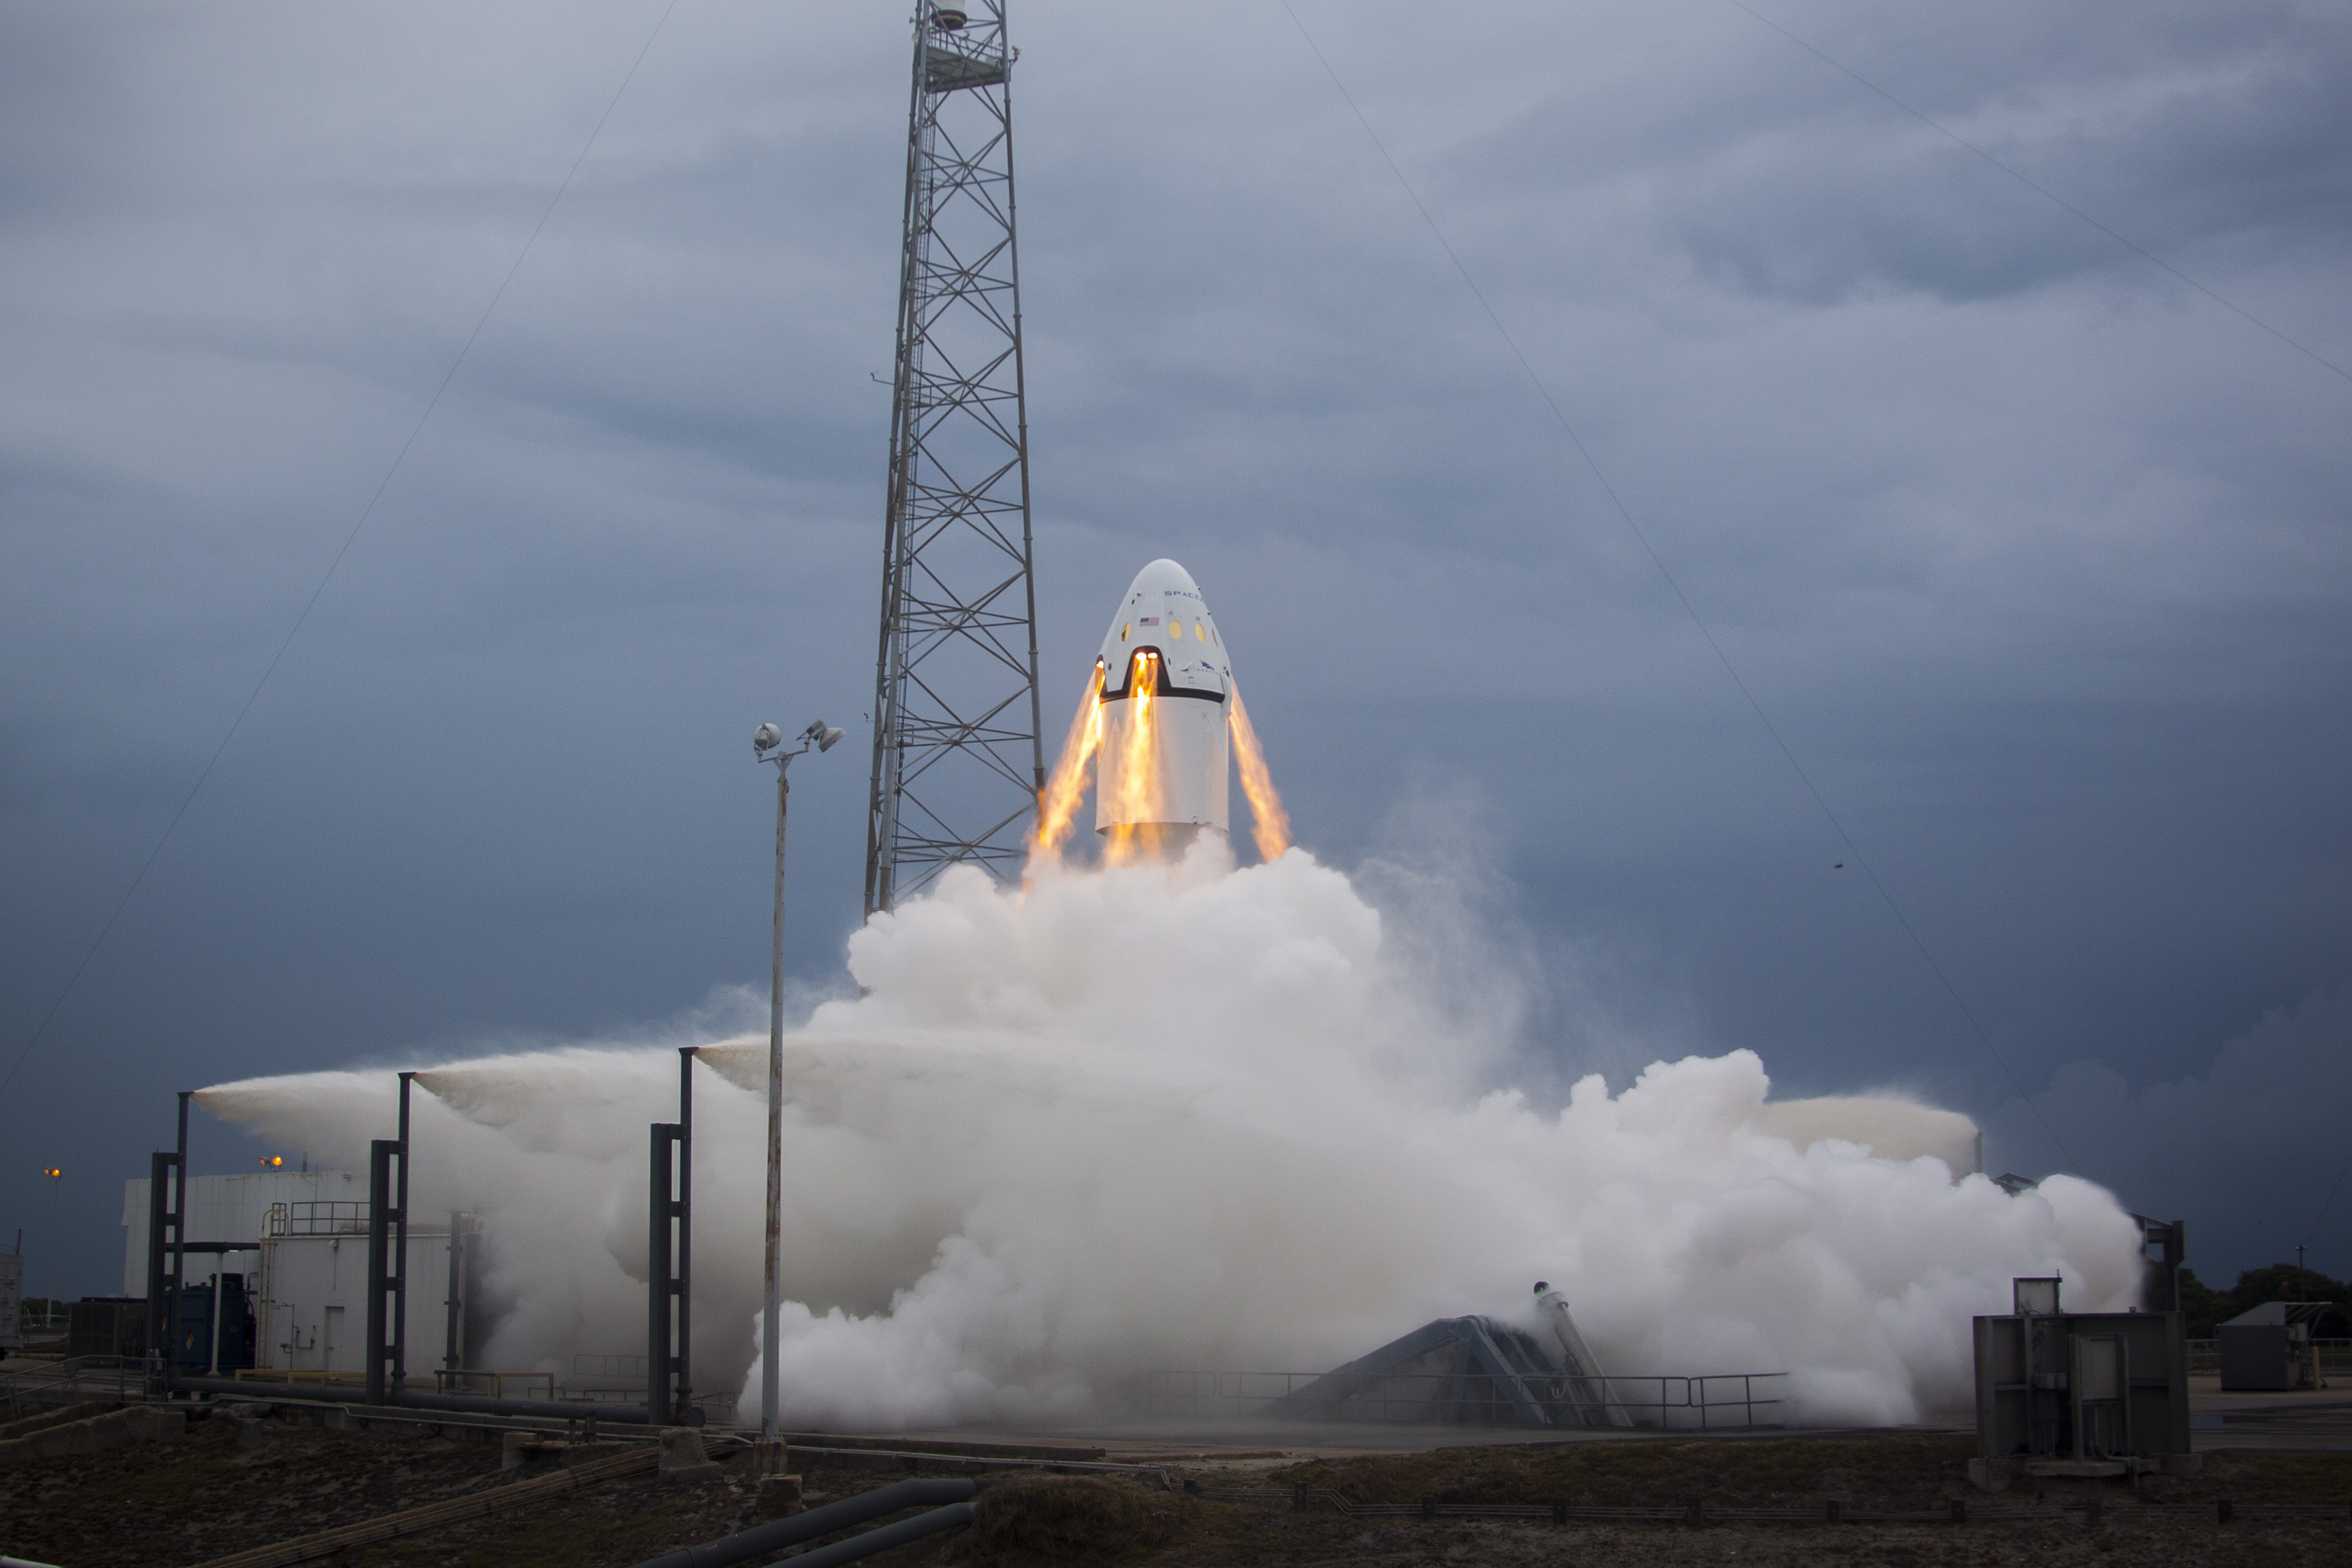
\includegraphics[width=0.9\textwidth]{Falcon9/dragon_pad_abort_launch2.jpg} 
    \caption{Pad abort testing. The maximum acceleration experienced by the Dragon capsule during an abort test is $\approx 6g$. Image from \cite{SpaceXPhotos}.}
    \label{fig:PadAbort}
\end{figure}

\section{Measured performance}

In order to verify the physics model, it must be compared against real world data. Because the true flight performance is strictly proprietary and confidential, the publicly released videos and associated commentary of three different launches were transcribed. This measured performance closely correlated with the modelled performance of the Falcon9 V1.1, and formed the basis for the design of the simulations utilised. 

\begin{table}[!htb]
\centering
\begin{tabular}{|l|l|}
\hline
\rowcolor[HTML]{C0C0C0} 
Time (s) & Event                                \\ \hline
60       & 5.8km alt, 250m/s, 0.8km down range  \\ \hline
\rowcolor[HTML]{EFEFEF} 
86       & Max Q                                \\ \hline
127      & 38km alt, 1160m/s, 19km down range   \\ \hline
\rowcolor[HTML]{EFEFEF} 
150      & 61km alt, 1900m/s, 40km down range   \\ \hline
169      & Stage 1 separation                   \\ \hline
\rowcolor[HTML]{EFEFEF} 
180      & 93km alt, 2120m/s, 79km down range   \\ \hline
265      & 156km alt, 2500m/s, 193km down range \\ \hline
\rowcolor[HTML]{EFEFEF} 
380     & 202km alt, 3700m/s, 420km down range \\ \hline
454      & 210km alt, 4700m/s, 610km down range \\ \hline
\rowcolor[HTML]{EFEFEF} 
540      & 207km alt, 6700m/s, 925km down range \\ \hline
\end{tabular}
\caption{CRS-4 flight transcript \cite{CRS4}.}
\label{tab:CRS4}
\end{table}
\begin{table}[!htb]
\centering
\begin{tabular}{|l|l|}
\hline
\rowcolor[HTML]{C0C0C0} 
Time (s) & Event                                \\ \hline
60       & 5.5km alt, 250m/s 0.9km down range   \\ \hline
\rowcolor[HTML]{EFEFEF} 
97       & Max Q                                \\ \hline
126      & 35km alt, 1000m/s 14.5 km down range \\ \hline
\rowcolor[HTML]{EFEFEF} 
150      & 58km alt, 1800m/s 33 km down range   \\ \hline
165      & Stage 1 seperation                   \\ \hline
\rowcolor[HTML]{EFEFEF} 
185      & 90km alt, 1900m/s 67km down range    \\ \hline
240      & 134km alt, 2100m/s, 135km down range \\ \hline
\rowcolor[HTML]{EFEFEF} 
270      & Stage 1 boost-back start             \\ \hline
300      & 166km alt, 2600m/s                   \\ \hline
\rowcolor[HTML]{EFEFEF} 
316      & Stage 1 boost-back stop              \\ \hline
412      & Stage 1 entry burn start             \\ \hline
\rowcolor[HTML]{EFEFEF} 
428      & Stage 1 entry burn stop              \\ \hline
435      & 205km alt, 4200km, (garbled) down range    \\ \hline
\rowcolor[HTML]{EFEFEF} 
475      & Stage 1 transonic                    \\ \hline
514      & Stage 1 under horizon                \\ \hline
\rowcolor[HTML]{EFEFEF} 
540      & 208km, 6900m/s 850km down range      \\ \hline
565      & Stage 2 engine shutdown              \\ \hline
\end{tabular}
\caption{CRS-5 flight transcript \cite{CRS5}.}
\label{tab:CRS5}
\end{table}
\begin{table}[!htb]
\centering
\begin{tabular}{|l|l|}
\hline
\rowcolor[HTML]{C0C0C0} 
Time (s) & Event                                 \\ \hline
120      & 32km alt, 1000m/s, 13.5km down range  \\ \hline
\rowcolor[HTML]{EFEFEF} 
165      & Stage seperation                      \\ \hline
180      & 86km alt, 1950m/s, 63km down range    \\ \hline
\rowcolor[HTML]{EFEFEF} 
277      & Stage 1 boost-back start              \\ \hline
300      & 165km alt, 2560m/s, 212km down range  \\ \hline
\rowcolor[HTML]{EFEFEF} 
315      & Stage 1 boost-back stop               \\ \hline
405      & Stage 1 entry burn start              \\ \hline
\rowcolor[HTML]{EFEFEF} 
425      & Stage 1 entry burn stop               \\ \hline
450      & 205km alt, 4400m/s, 530km down range  \\ \hline
\rowcolor[HTML]{EFEFEF} 
491      & Stage 1 transonic                     \\ \hline
540      & 208 km alt, 6500m/s, 830km down range \\ \hline
\rowcolor[HTML]{EFEFEF} 
574      & Stage 2 shutdown \\ \hline
\end{tabular}
\caption{CRS-6 flight transcript \cite{CRS6}.}
\label{tab:CRS6}
\end{table}

\clearpage
\section{Velocity requirements}
The 2nd stage burn must be terminated at precisely the right time, to ensure that the final velocity is correct. This is because the orbital height is dictated by the velocity, 

\begin{equation}
v_0 = \sqrt{\frac{G \cdot M}{r}}
\end{equation}

Where:
\begin{align*}
G &= 6.673 \times 10^{-11} N m^2 kg^{-2}\\
M &= 5.972 \times 10^{24} kg
\end{align*}

\begin{equation}
r = \frac{G \cdot M}{v_0^2}
\end{equation}

\begin{equation}
\frac{dr}{dv} = \frac{-2 \cdot G \cdot M}{v_0^3}
\end{equation}

For \ac{LEO}, with an orbital velocity of $\approx$ 7,800 m/s, this results in a a differential of 1,679m of altitude, per m/s of velocity. Given that SpaceX guarantees orbital height of $\pm$ 10km, this results in a velocity tolerance of $\pm$ 5.95 m/s, or $\pm$ 31.2 Hz of doppler shift. 

Using a nominal value of \$5,000 USD for each Kg of cargo delivered to \ac{LEO}, and with a fuel burn rate of 250Kg/s, every second of additional carries an opportunity cost of \$1.25M USD. Given any mistake in velocity requires a burn of approximately equal duration to correct, Each m/s of velocity error costs \$50,000 to rectify. Accelerating at a nominal rate of 50 m/s, this equates to a timing error of 100ms. Based on this information, it can be concluded that the receiver should produce velocity estimates which are accurate to $\leq$ 1m/s.

\begin{table}[!htb]
\centering
\begin{tabular}{|l|l|l|l|l|l|}
\hline
\rowcolor[HTML]{C0C0C0} 
Date      & Vehicle       & No    & Payload      & Mass (Tons)         & Orbit                  \\ \hline
21/9/2014 & Falcon 9 v1.1 & F9-13 & CRS-4 Dragon & $\approx$ 9.3  & 199x359x51.64  LEO/ISS \\ \hline
\rowcolor[HTML]{EFEFEF} 
10/1/2015 & Falcon 9 v1.1 & F9-14 & CRS-5 Dragon & $\approx$ 9.54 & 206x353x51.6 LEO/ISS   \\ \hline
14/5/2015 & Falcon 9 v1.1 & F9-18 & CRS-6 Dragon & $\approx$ 9.24 & 199x364x51.65  LEO/ISS \\ \hline
\end{tabular}
\caption{Falcon 9 V1.1 missions to the ISS.}
\label{tab:Falcon9Missions}
\end{table}
\cite{Falcon9Stats}

\begin{table}[!htb]
\centering
\begin{tabular}{|l|l|}
\hline
\rowcolor[HTML]{C0C0C0} 
Time (s) & Event                                     \\ \hline
0.0      & Liftoff from Cape Canaveral               \\ \hline
\rowcolor[HTML]{EFEFEF} 
7.5      & Initial Pitch Kick                        \\ \hline
55.0     & Begin gravity turn                        \\ \hline
\rowcolor[HTML]{EFEFEF} 
76.0     & Max-Q                                     \\ \hline
115.0    & Release angle of attack restrictions      \\ \hline
\rowcolor[HTML]{EFEFEF} 
155.5    & Shutdown 2 engines for acceleration limit \\ \hline
174.2    & Main Engine Cut Off                       \\ \hline
\rowcolor[HTML]{EFEFEF} 
176.2    & Stage 1/Stage 2 separation                \\ \hline
179.2    & Second stage engine start \#1             \\ \hline
\rowcolor[HTML]{EFEFEF} 
199.2    & Payload fairing jettison                  \\ \hline
475.9    & Second stage engine cut off               \\ \hline
\end{tabular}
\caption{Falcon 9 sample flight time-line \cite{Falcon9}.}
\label{tab:Falcon9Timeline}
\end{table}


\begin{figure}[!htb] 
    \centering
    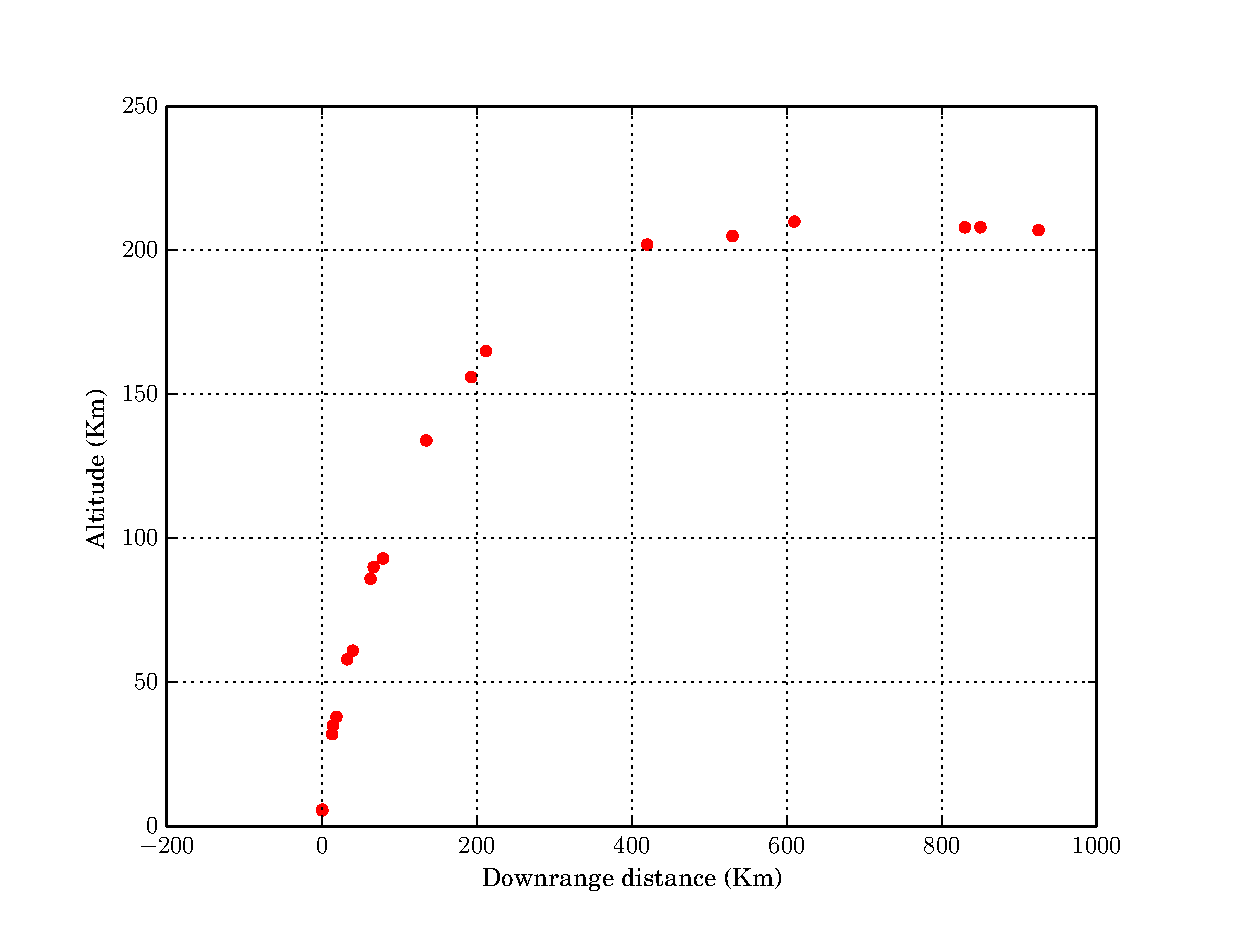
\includegraphics[width=1\textwidth]{Falcon9/FlightProfile.eps} 
    \caption{The Falcon 9 V1.1 flight profile, compare with figure \ref{fig:Falcon9Launch}.}
    \label{fig:Falcon9FlightProfile}
\end{figure}


\begin{figure}[!htb] 
    \centering
    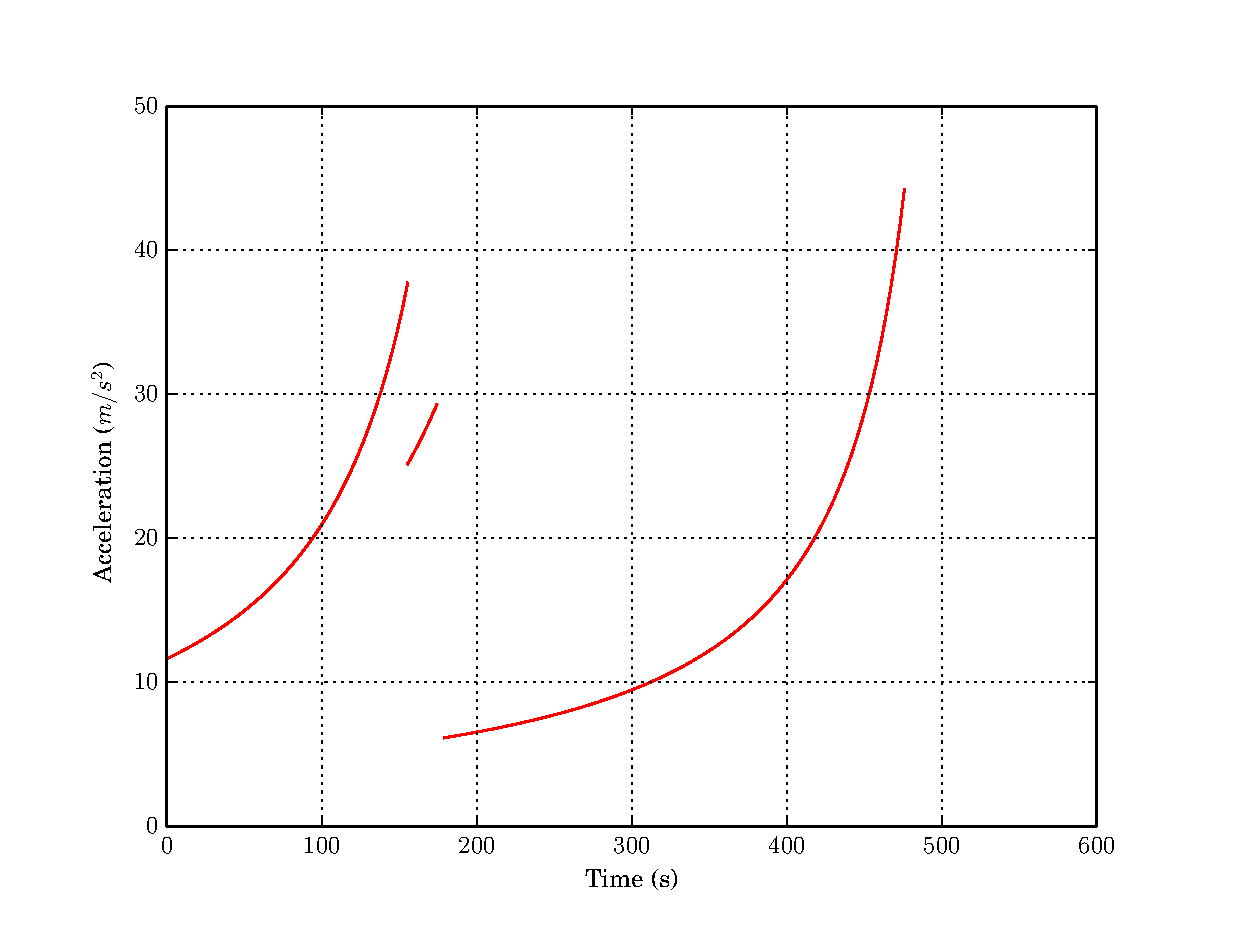
\includegraphics[width=1\textwidth]{Falcon9/Model.eps}
    \caption{The modelled acceleration performance. This performance was estimated based on the physical parameters of the vehicle, and should be treated as representative, rather than authoritative.}
    \label{fig:Falcon9Model}
\end{figure}


\begin{figure}[!htb] 
    \centering
    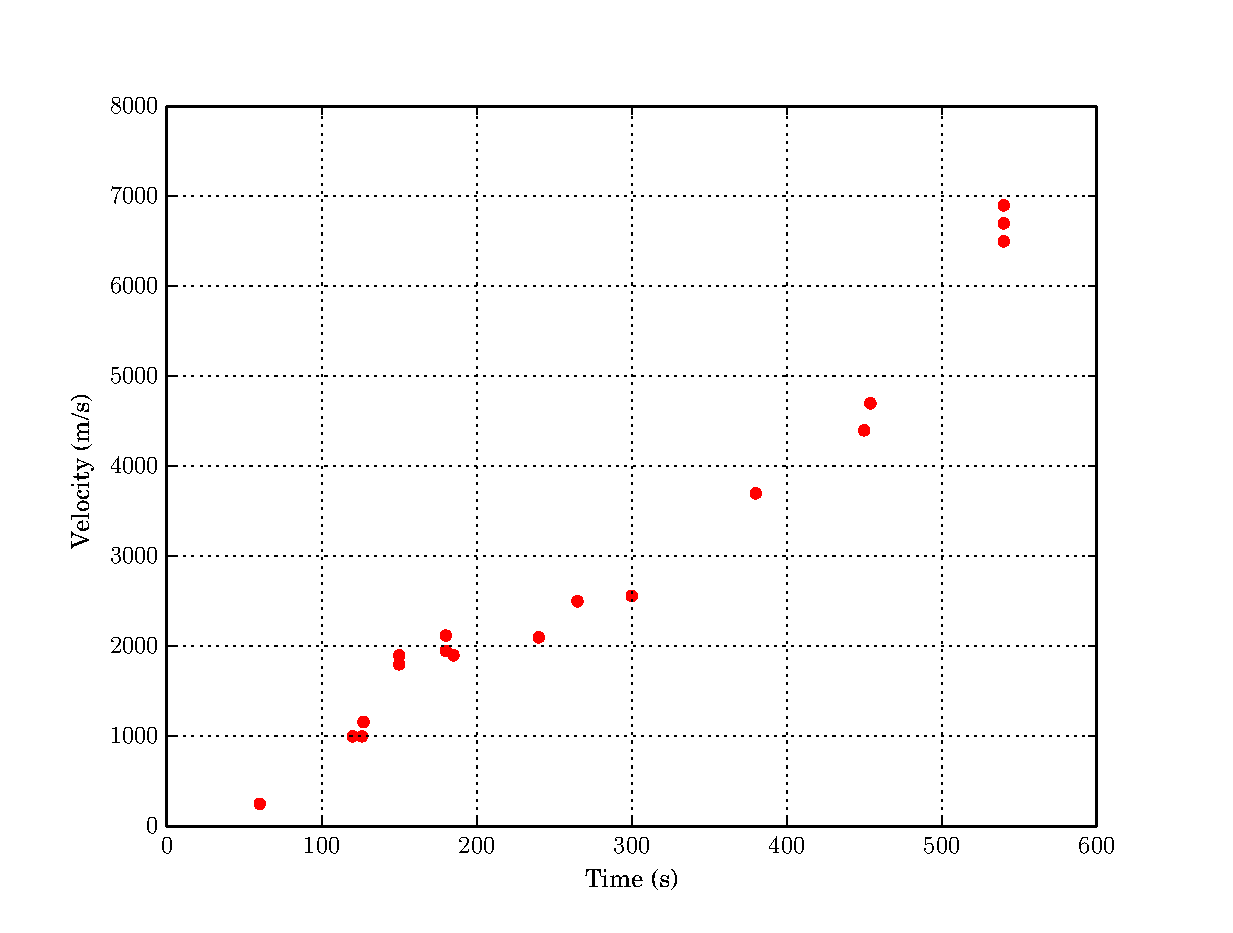
\includegraphics[width=1\textwidth]{Falcon9/VelocityProfile.eps}
    \caption{The measured flight velocity from launches CRS-4 to CRS-6. Note the exponential increase in velocity, as as the rocket burns fuel over time.}
    \label{fig:Falcon9VelocityProfile}
\end{figure}



\begin{figure}[!htb] 
    \centering
    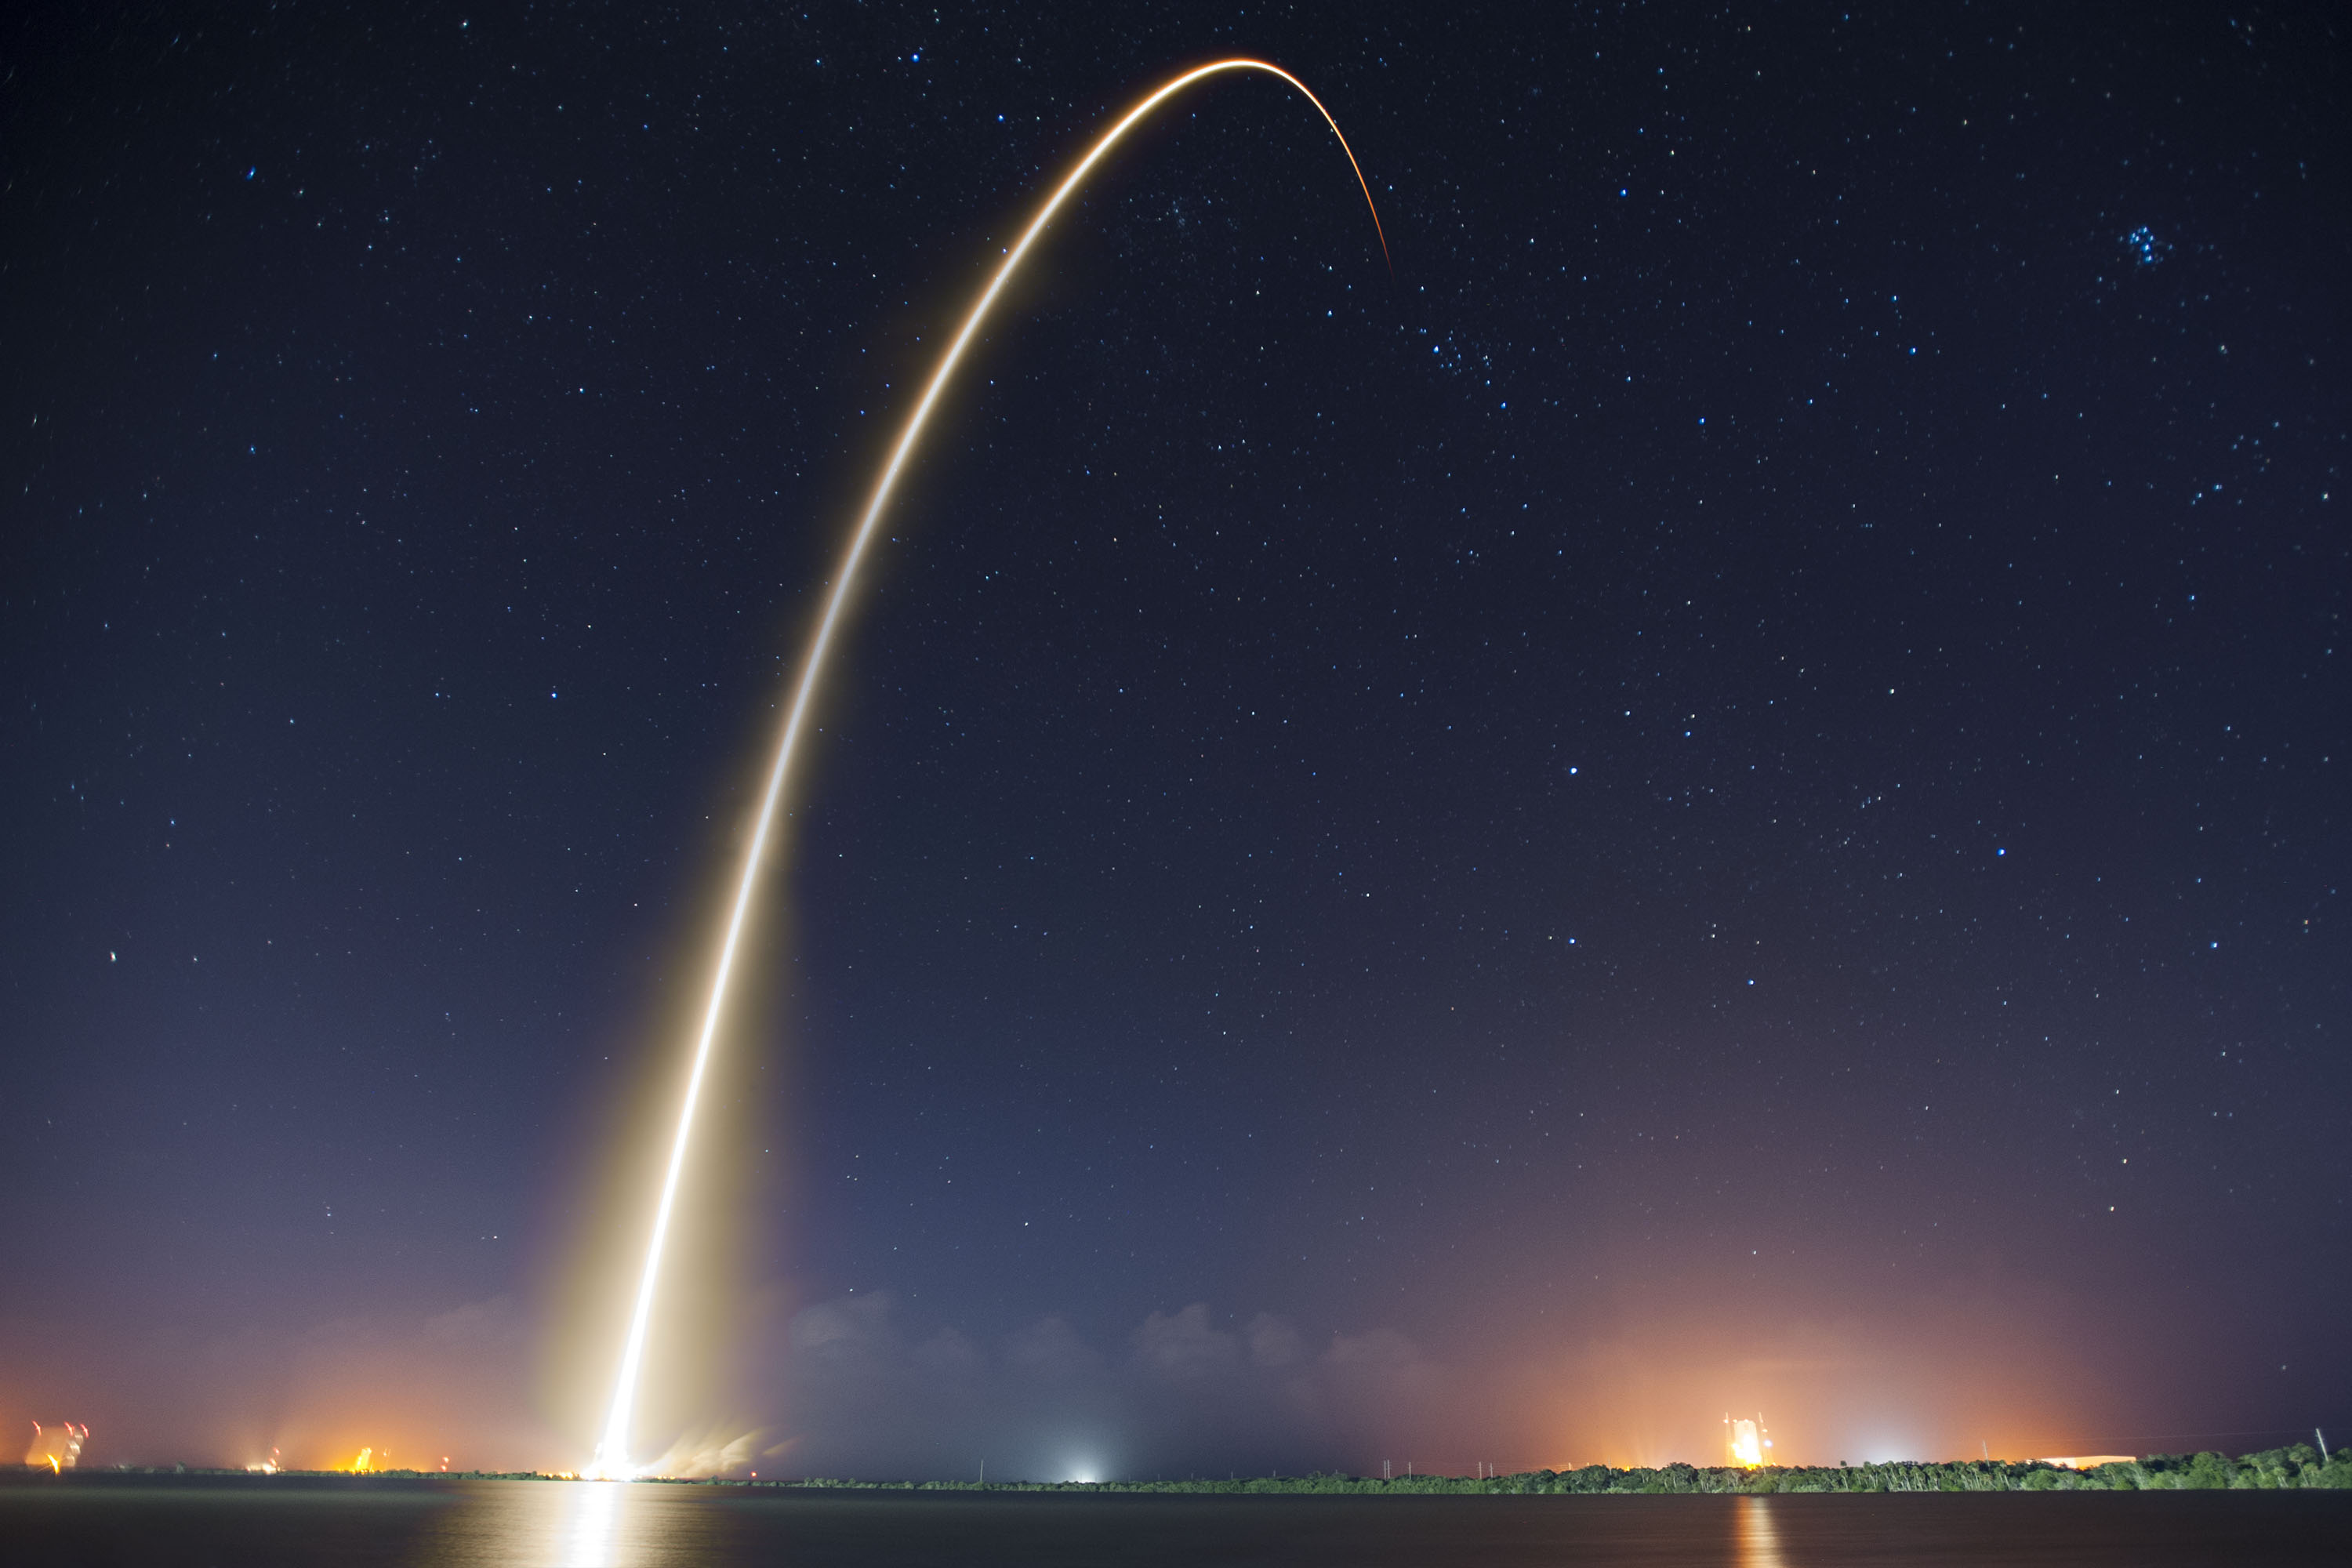
\includegraphics[width=1\textwidth]{Falcon9/Launch1.jpg}
    \caption{An oblique view of a Falcon 9 V1.1 launch \cite{SpaceXPhotos}.}
    \label{fig:Falcon9Launch}
\end{figure}

\clearpage
\section{Launch azimuth}

\begin{equation}
\beta = arcsin \Big(\frac{cos(i)}{cos(\phi)}\Big)
\end{equation}

Where:
\begin{align*}
 i &= \text{Orbit inclination}\\
 \phi &= \text{Launch site latitude}\\
 \beta &= \text{Launch azimuth}\\
\end{align*}


The \ac{ISS} has an inclination of $51.6\degree$, hence a launch from Cape Canaveral ($\phi = 28.5\degree$), $\beta=44.9\degree$\cite{LaunchDesign}.


\begin{figure}[!htb] 
    \centering
    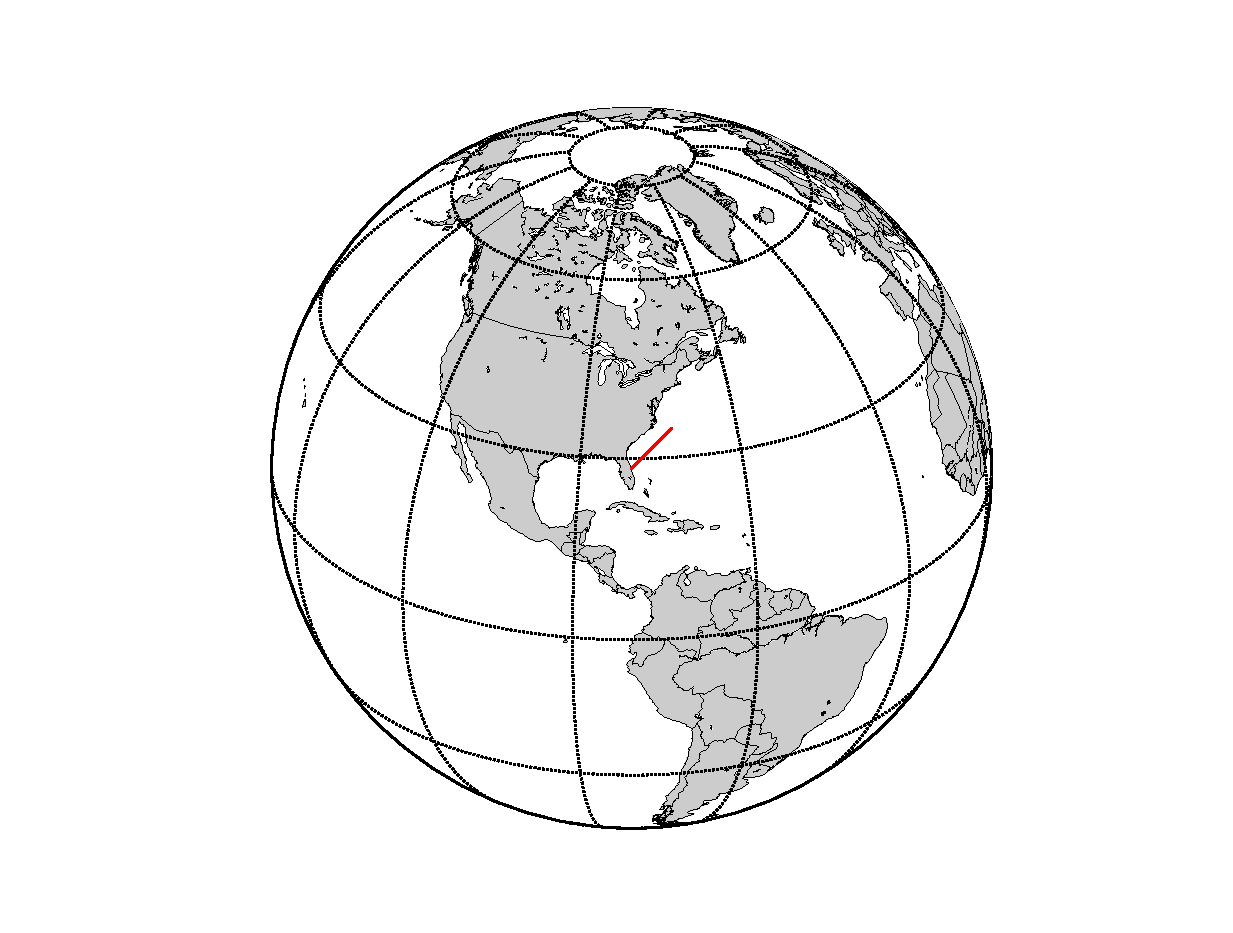
\includegraphics[width=1\textwidth]{Falcon9/CapeCanaveral.eps}
    \caption{}
    \label{fig:LaunchPath}
\end{figure}


\begin{comment}
\begin{figure}[!htb] 
    \centering
    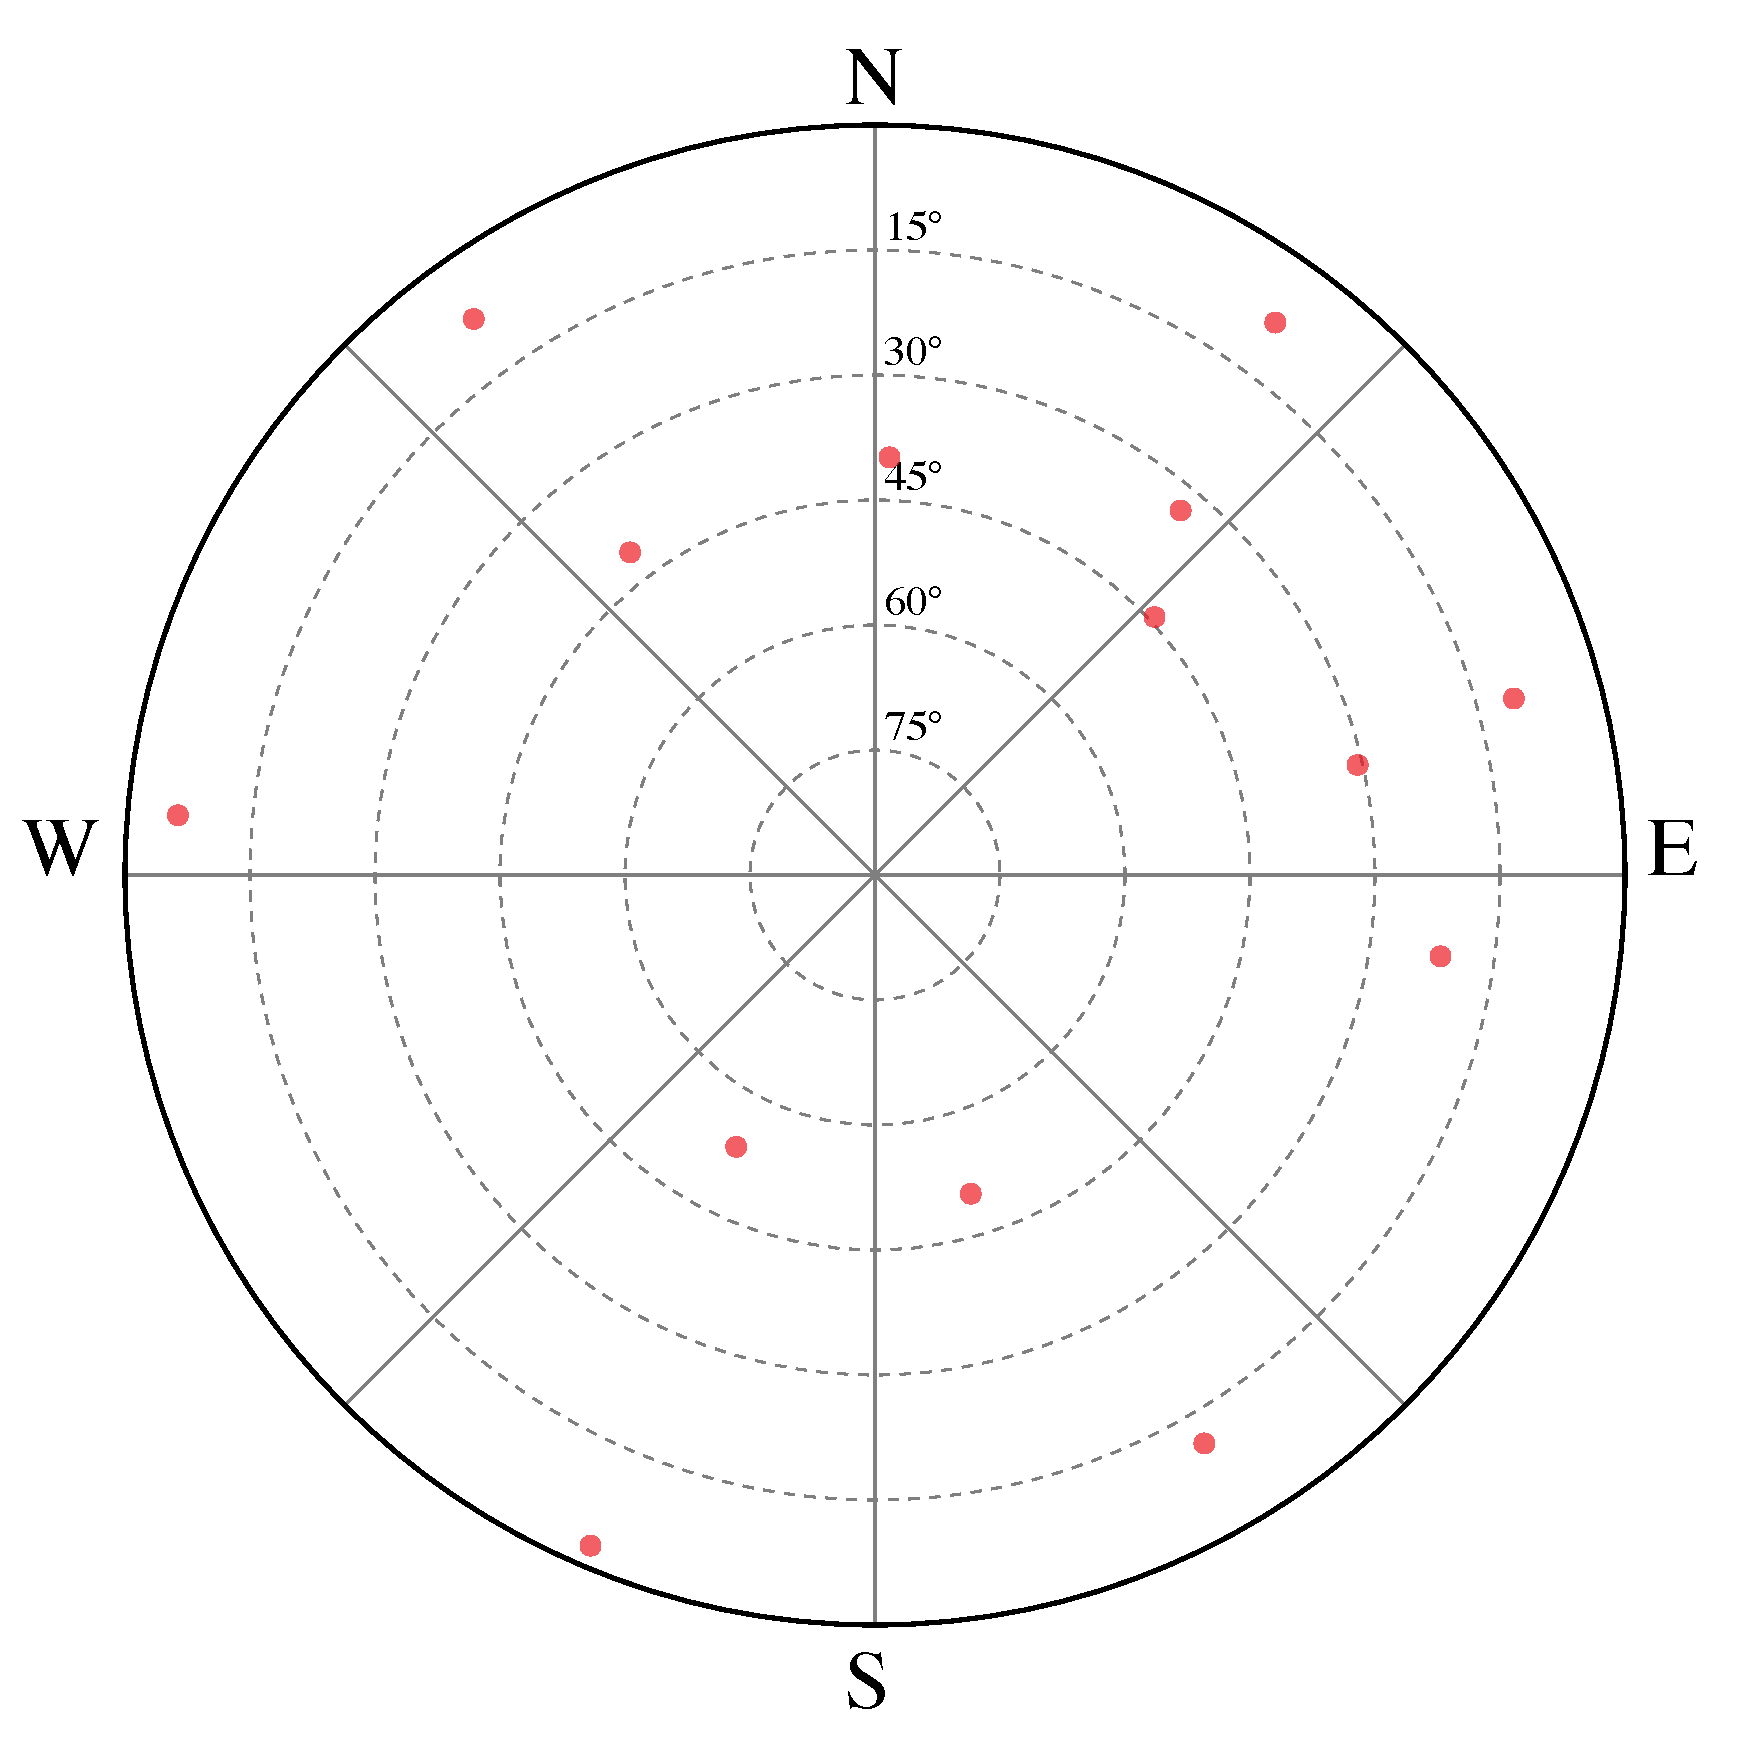
\includegraphics[width=1\textwidth]{Falcon9/Skyplot.pdf}
    \caption{}
    \label{fig:Skyplot}
\end{figure}
\end{comment}

\clearpage
\section{Burn-back procedure}

Space Exploration Technologies Corporation (SpaceX) is attempting to reduce launch costs by recovering the first stage of their Falcon 9-R launch vehicle. After first stage separation, the first stage performs a burn-back procedure, to fly back to the launch pad\cite{SpaceXFalcon9}. Given the primary goal of any launch is to deliver the maximum amount of payload to orbit optimisation of the fuel burn is critical. For context, of the gross mass of the launch vehicle, only $\approx$ 2\%  is revenue earning payload. By safely returning the 1st stage, with a nominal value of \$50M, significant savings can be achieved. An overview of the flight profile can be found in figure \ref{fig:Falcon9Profile}.


\begin{figure}[!htb] 
    \centering
    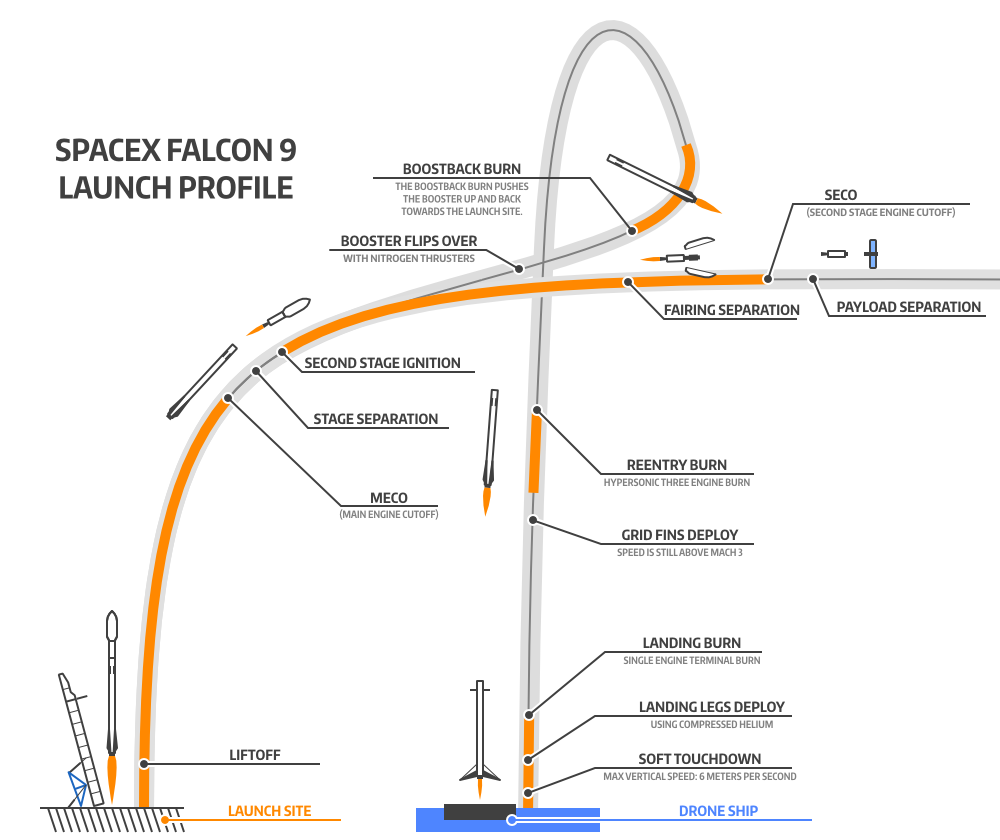
\includegraphics[width=1\textwidth]{FlightDynamics/Falcon9Profile.png} 
    \caption{An overview of the Falcon 9-R flight profile.}
    \label{fig:Falcon9Profile}
\end{figure}


The Burn-back procedure requires exquisite timing precision and velocity accuracy for guidance. The most fuel efficient method of returning a rocket to earth is to perform the de-acceleration burn at the last possible moment, at the highest rate possible. The rationale behind this procedure, is that it reduces the flight time, minimising the total downward velocity imparted on the rocket due to gravity. 

Three separate burns are uses as part of the burn-back procedure. The boost-back burn provides gross guidance of the 1st stage towards the landing zone. The hypersonic re-entry burn reduces the velocity from 1300 m/s to  250 m/s using 3 engines. The landing burn slows the 1st stage to 0/ms, at 0 m altitude using a single engine. This sequence can be clearly seen in figure \ref{fig:Falcon9Profile}.

While this method optimises the fuel consumption of the rocket, it also minimises the margin for error. If the downward velocity of the rocket is under-estimated, then the rocket will collide with the pad at speed, resulting in the total loss of the \ac{LV}.  To further complicate matters, very little fuel remains in the 1st stage just prior to landing, due to the opportunity cost of carrying un-burned fuel. The Falcon 9 V1.1 R 1st stage has a dry weight of 25.6 tons, each Merlin 1D engine has a rated thrust sea level thrust of of 756Kn, or 66.73 tons. Hence as the 1st stage consumes fuel, it's thrust/weight ratio approaches 2.6. 

Because of the positive thrust/weight ratio, once the rocket's vertical velocity has come to zero, it will continue to accelerate upwards unless the throttle is brought to zero. To make the process significantly more complex, that engine can only be throttled between 70-100\% thrust. Even with 70\% throttle, the 1st stage is accelerating upwards at $\approx$ 8.0m/s. Hence, accurate estimates of velocity and position are critical to reliably bring the 1st stage to rest at sea level. An un-successful attempt at this manoeuvre can be seen in figure \ref{fig:Kaboom}.

During the burn-back, there is an inferred maximum de-acceleration of $\approx 6.8 g$ during the hypersonic burn, based on published performance figures. This figure can be arrived based on use of 3 engines during the hypersonic re-entry burn. 


\begin{figure}[!htb] 
    \centering
    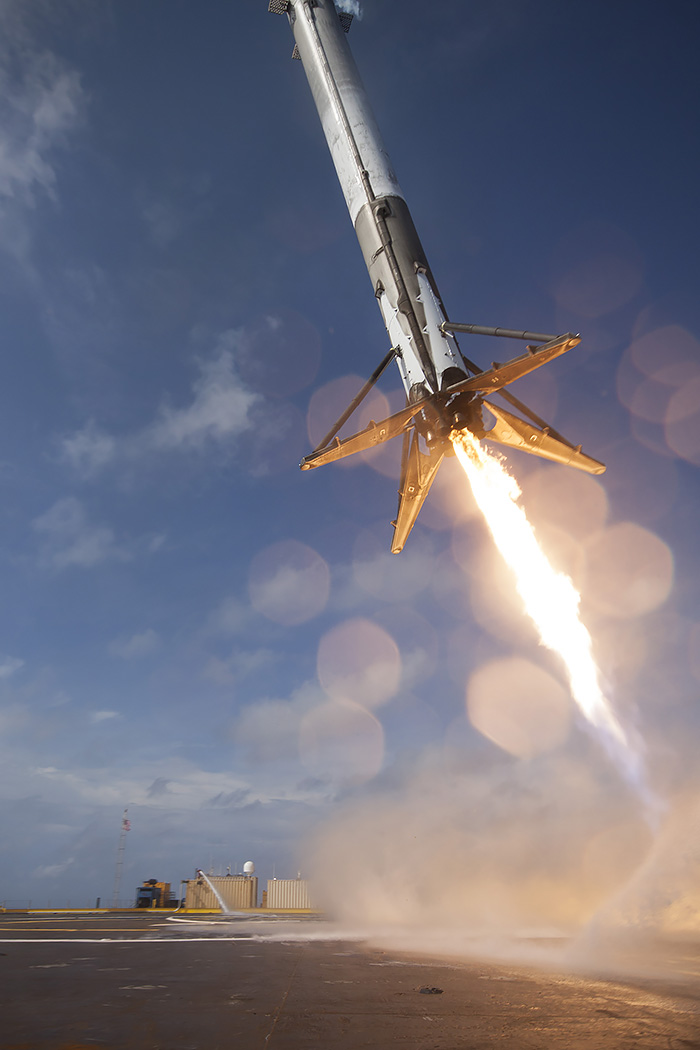
\includegraphics[width=0.8\textwidth]{Falcon9/CRS6Landing.jpg} 
    \caption{The CRS-6 1st stage landing attempt. A phase lag in the throttle control loop resulted in unstable behaviour culminating in the  loss of the vehicle in addition to significant damage to the landing pad \cite{SpaceXPhotos}.}
    \label{fig:Kaboom}
\end{figure}


